\documentclass[9pt,lineno]{elife}

%%%%%%%%%%%%%%%%%%%%%%%%%%%%%%%%%%% table
\usepackage{multirow}

%%%%%%%%%%%%%%%%%%%%%%%%%%%%%%%%%% font size %%%%%%%%%%%%%%%%%%%%%%%%
\usepackage{anyfontsize}

%%%%%%%%%%%%%%%%%%%%%%%%%%%%%%%%%% Maths %%%%%%%%%%%%%%%%%%%%%%%%%%%%
\usepackage{amsmath}

%%%%%%%%%%%%%%%%%%%%%%%%%%%%%%%%%% referencing %%%%%%%%%%%%%%%%%%%%%%%%%%%%%%%%%%
%\usepackage{natbib}
\usepackage{hyperref}
\usepackage{xcolor}
\hypersetup{
    colorlinks,
    %linkcolor={red!50!black},
    linkcolor={black},
    citecolor={blue!50!black},
    urlcolor={blue!80!black}
}

%%%%%%%%%%%%%%%%%%%%%%%%%%%%%%%%%% figure and table %%%%%%%%%%%%%%%%%%%%%%%%%%%%%%%%%%
\usepackage{graphicx}
\graphicspath{{./figures/}}
%\graphicspath{{}}
\usepackage[label font=bf,labelformat=simple, position = top]{subfig}
\newdimen\figrasterwd
\figrasterwd\textwidth
\usepackage{wrapfig}
\usepackage{lipsum}

%%%%%%%%%%%%%%%%%%%%%%%%%%%%%%%%%% layout %%%%%%%%%%%%%%%%%%%%%%%%%%%%%%%%%%
\usepackage{setspace}
\linespread{1.5}
\usepackage{authblk}

%\usepackage{fancyhdr}
\providecommand{\keywords}[1]{\textbf{\textit{Key words:}} #1}

%\newcommand\@shorttitle{}
% define \theshorttitle to what is given
%\newcommand\shorttitle[1]{\renewcommand\@shorttitle{#1}}

%%%%%%%%%%%%%%%%%%%%%%%%%%%%%%%%%% todo %%%%%%%%%%%%%%%%%%%%%%%%%%%%%%%%%%
%\usepackage[colorinlistoftodos]{todonotes}
\usepackage[disable]{todonotes}

\newcounter{todocounter}
\newcommand{\todonum}[2][]
{\stepcounter{todocounter}\todo[#1]{\thetodocounter: #2}}

\newcommand{\done}[2][]
{\todo[color=green!40, #1]{#2}}
\newcommand{\donenum}[2][]
{\stepcounter{todocounter}\done[#1]{\thetodocounter: #2}}


\newcommand{\narrative}[2][]
{\todo[color=blue!40, #1]{#2}}
\newcommand{\narrativenum}[2][]
{\stepcounter{todocounter}\narrative[#1]{\thetodocounter: #2}}

\newcommand{\donenarrative}[2][]
{\todo[color=green!40, #1]{#2}}
\newcommand{\donenarrativenum}[2][]
{\stepcounter{todocounter}\narrative[#1]{\thetodocounter: #2}}



\begin{document}

\title{Characterising local epidemiology of {\it P. falciparum} malaria through the structure of mixed infections}
\newcommand\shorttitle{Mixed infections in malaria}
\date{}

\author[?]{(LIST OF NAMES, NEEDS ORDERING)}
\author[1]{Sha Joe Zhu}
\author[1,2,3,4]{Jacob Almagro-Garcia}
\author[1]{Jason Hendry}
\author[2,3]{Richard Pearson}
\author[2,3]{Alistair Miles}
\author[2,3]{Roberto Amato}
\author[?]{Pf3k Consortium}
\author[2,3]{Dominic Kwiatkowski}
\author[1,3]{Gil McVean}

\corr{gil.mcvean@bdi.ox.ac.uk}{GM}

\affil[1]{Big Data Institute, Li Ka Shing Centre for Health Information and Discovery, University of Oxford, Oxford, UK}
\affil[2]{Wellcome Centre for Human Genetics, University of Oxford, Oxford, UK}
\affil[3]{Medical Research Council (MRC) Centre for Genomics and Global Health, University of Oxford, Oxford, UK}
\affil[4]{Wellcome Trust Sanger Institute, Hinxton, UK}
%\donenum[inline]{updated affiliation}
%}

\maketitle{}

\begin{abstract}
{\it Plasmodium falciparum} infections can be caused by multiple strains with a distinct genetic makeup. Within mixed infections, these genetic types can exhibit different levels of relatedness. However, how the rate and relatedness of such infections influence local epidemiological parameters remains unclear.  Here, we develop an enhanced method for strain deconvolution from genome sequencing data, which estimates the number of strains, their proportions, relatedness profiles and individual haplotypes.  We validate the method via simulations and controlled experiments, and apply it to Pf3k data set, consisting of 2,344 isolates from 13 countries.  Rates of mixed infection vary from 18\% to 63\% across countries and correlate with independent estimates of parasite prevalence (Pearson $r = 0.59$, P$=3.8e-6$).  51\% of mixed infections involve more than two strains whereas 47\% include sibling strains likely to have been co-transmitted from a single mosquito. We found that relatedness among strains decreases with prevalence ($r = -0.43$, P$=3.0e-3$) and differs between continents, with Asian isolates typically showing higher relatedness than their African counterparts.Capitalising on \textit{in silico} simulations, we classify isolates carrying two strains according to the most likely number of meiosis that separate them. We conclude that monitoring spatial and temporal patterns of mixed infection and relatedness between strains will be highly informative in pathogen surveillance and assessment of interventions.
\end{abstract}

\keywords{Malaria, genome, epidemiology, relatedness}


\section{Introduction}


Individuals infected with malaria-causing parasites of the genus {\it Plasmodium} often carry multiple, distinct strains of the same species ~\citep{Bell2006}.  Such mixed infections are likely indicative of intense local exposure rates, being common in regions of Africa with high rates of prevalence~\citep{Bhatt2015, Howes2016}. However, they have been documented for {\it P.~vivax} and other malaria-causing parasites~\citep{Mueller2007, Collins2012}, even in regions of much lower prevalence~\citep{Howes2016, Steenkeste2010}.  For example, \citet{Pearson2016} reports 45\% of {\it P.~vivax} infections carry more than one genetic type.  Mixed infections have been associated with increased disease severity \citep{deRoode2005} and also facilitate the generation of genomic diversity within the parasite, enabling co-transmission to the mosquito vector where sexual recombination occurs \citep{Mzilahowa2007}.  Mixed infections are transient \citep{Bruce2002, Zimmerman2004}, but little is known about the distribution of their duration. Whether the clearance of one or more strains results purely from host immunity~\citep{Borrmann2011} or can be influenced by interactions between the distinct strains~\citep{Enosse2006, Bushman2016}, are also open questions.

Although mixed infections can be studied from genetic barcodes~\citep{Galinsky2015} or single nucleotide polymorphisms (SNPs)~\citep{Jack2016}, genome sequencing provides a more powerful approach for detecting mixed infections~\citep{Chang2017}.  Genetic differences between co-existing strains manifest as polymorphic loci in the sequence of the isolate. The higher resolution of sequencing data allows the use of statistical methods for estimating the number of distinct strains, their relative proportions, and genome sequences~\citep{Zhu2017}.  Although genomic approaches cannot identify individuals infected multiple times by identical strains, and are affected by sequencing errors and problems of incomplete or erroneous reference assemblies, they provide a rich characterisation of within host diversity~\citep{Manske2012}.

Previous research has highlighted that co-existing strains can be highly related~\citep{Nair2014, Trevino2017}.  For example, in {\it P. vivax}, 58\% of mixed infections show long stretches of within host homozygosity~\citep{Pearson2016}. In addition, \citet{Nkhoma2012} reported an average of 78.7\% {\it P. falciparum} allele sharing in Malawi and 87.6\% sharing in Thailand. This could result from co-infection by sibling strains where a mosquito vector has acquired several strains from biting multiple infected individuals, a single individual infected by more than one strain, or a combination of the two.  Alternatively, higher levels of relatedness can occur when population diversity is low, such as during the early stages of an outbreak or following severe population bottlenecks. Extensive relatedness has also been observed at the population level.  For example, following a malaria control intervention in Senegal~\citep{Mouzin2010}, haplotype diversity within isolates decreased as a consequence of the induced population bottleneck~\citep{Wong2017}.

The rate and relatedness structure of mixed infections are clearly relevant for understanding regional epidemiology.  However, progress towards utilising this source of information is limited by three problems.  Firstly, while strain deconvolution within mixed infections has received substantial attention~\citep{Galinsky2015, Jack2016, Chang2017, Zhu2017}, joint deconvolution of strains and estimation of relatedness has not been attempted.  Because existing deconvolution methods assume equal relatedness along the genome, differences in relatedness that occur, for example, through infection by sibling strains can lead to errors in the estimation of the number, proportions and sequences of individual strains (Figure \ref{fig:fig1}).  Recently, progress has been made in the case of dual-infections with balanced proportions~\citep{Henden2016}, but a general solution is lacking.  The second limitation is that little is known about how the rate and relatedness structure of mixed infections relates to underlying epidemiological parameters.  Informally, mixed infections will occur when prevalence is high; an observation exploited by \citet{Cerqueira2017} when estimating changes in transmission over time.  However, the quantitative nature of this relationship, the key parameters that influence mixed infection rates and how patterns of relatedness relate to infection dynamics are largely unexplored.  Finally, an important, but often overlooked issue is the sampling design.  Malaria parasites may be taken from individuals presenting with disease or as part of a surveillance programme.  They are also often highly clustered in time and space.  What the impact of different approaches have on observed genomic variation is not clear.  Nevertheless, because mixed infection rates are likely to respond rapidly to changes in prevalence~\citep{volkman2012}, exploring these issues is an important task.

Here, we develop, test and apply an enhanced method for strain deconvolution, which builds on our previously-published \texttt{DEploid} software.  The method works by separating the process of estimating strain number, proportions, and relatedness (specifically the identity-by-descent, or IBD, profile along the genome) from the problem of inferring genome sequences. This new strategy provides substantial improvements in accuracy under complex settings or when dealing with low coverage data.  We apply this approach to 2,344 isolates of {\it P. falciparum} collected from 13 countries over a range of years [2001-2014], and characterise the rate and relatedness patterns of mixed infections.  We show that country-level rates of mixed infection are highly correlated with estimates of malaria parasite prevalence collected by the Malaria Atlas Project (MAP). Furthermore, we find that levels of IBD are negatively correlated with mixed infection rates, and hence parasite prevalence, but are also influenced by other aspects of local epidemiology, such as recent dramatic changes in transmission. For example, we observe a lower effective number of parasite strains within isolates in Senegal as compared to other Africa countries. 


\section{Strain deconvolution in the presence of relatedness}

Existing methods for deconvolution of mixed infections assume that the different genetic strains present in mixed infections are unrelated.  This assumption allows for efficient computation of priors for allele frequencies within samples, either through assuming independence of loci~\citep{Jack2016} or as sequences generated as imperfect mosaics of some (predefined) reference panel~\citep{Zhu2017}.  However, when strains are related to each other, certain allele frequencies are excluded; for example, within a region of IBD for a mixed infection with two strains, only allele frequencies of 0 and 1 are possible.  Because patterns of IBD are likely to vary along the genome, these constraints can cause problems for estimators, which can try to fit complex strain combinations (with relatedness) as simpler configurations (without relatedness).  Below we outline the approach taken to integrating IBD into \texttt{DEploid} and validate the approach.  Further details are provided in the Supplementary Materials.


\subsection{Decoding genomic relatedness among strains}

A common approach to detecting IBD between two genomes is to employ a hidden Markov Model that transitions into and out of IBD states~\citep{Chang2015, Gusev2009, Gusev2011}.  We have generalised this approach for the case of $k$ haploid {\it Plasmodium} genomes (strains). In this setting, there are $2^k$ possible genotype configurations, as each of the $k$ strains can be either reference, i.e. same as the reference genome used during assembly, or alternative at a given locus (we assume all variation is bi-allelic). If each of the $k$ strains constitutes a unique proportion of the infection (and no individual proportion is an additive combination of any of the rest), each genotype configuration will produce a distinct alternative allele frequency (Figure~\ref{fig:fig1}a). This frequency is observed as the fraction of total sequencing reads that are alternative at a given locus in the sequenced infection.

The effect of IBD among these $k$ strains is to limit the number of distinct genotype configurations possible, in a way that depends on the pattern of IBD sharing. Consider that, for any given locus, the $k$ strains in the infection are assigned to $j \leq k$ possible reference haplotypes. IBD exists when two or more strains are assigned to the same haplotype. Under this scenario, the total number of possible patterns of IBD sharing for a given $k$ is equal to $\sum_{j=1}^{k} S(k,j)$ where $S(k,j)$ is the number of ways $k$ objects can be split into $j$ subsets (a Stirling number of the second kind \citep{Ronald1988}). Thus, for two strains, there are two possible IBD patterns (IBD, or not), for three there are five configurations (all IBD, none IBD; plus each pairwise IBD possibility), for four there are fifteen configurations, and so on. We omit infections with greater than four strains for reasons of computational efficiency and because they are rarely observed. Finally, for a given IBD sharing pattern, only $2^j$ rather than $2^k$ genotype configurations are possible, thereby restricting the set of alternative allele frequencies.

Recombination can change the pattern of IBD sharing, and hence the alternative allele frequencies, along the genome (Figure~\ref{fig:fig1}b).  For inferring patterns of IBD we assume linkage equilibrium between variants, which speeds up computation, and use a Gamma-Poisson emission model for read counts (see Supplementary Methods).  Population-level allele frequencies are estimated from isolates obtained from a similar geographic region.  Because of the structure of the hidden Markov model, we can compute the likelihood of the strain proportions by integrating over all possible IBD sharing patterns.  Once the number and strain proportions have been estimated, we can then use maximum likelihood and posterior decoding to infer the relatedness structure across the genome (Figure~\ref{fig:fig1}b).

Unlike our previous work, \texttt{DEploidIBD} infers strain structure in two steps.  In the first we estimate the number and proportions of strains using Markov Chain Monte-Carlo (MCMC), allowing for IBD as described above.  In the second, we infer the individual genomes of the strains, using the MCMC methodology of~\citet{Zhu2017}, which can account for linkage disequilibrium (LD) between variants, but without updating strain proportions.


\begin{figure}[ht]
  \begin{center}
    \includegraphics[width=\textwidth]{Fig1.pdf}
    \caption{Deconvolution of a complex field sample PD0577-C from Thailand.  (a) Summary of allele frequencies observed within the isolate shown as a scatter-plot of the numbers of reads supporting the reference (REF: x-axis) and alternative (ALT: y-axis) alleles. The multiple clusters indicate several strains, but cannot distinguish the exact number or proportions.  (b) The profile of within-sample allele frequency along chromosomes 11 and 12 (red points) suggests a changing profile of IBD with three distinct strains, estimated to be with proportions of $22\%$, $52\%$ and $26\%$ respectively (other chromosomes omitted for clarity, see Figure~\ref{fig:fig1}-Supplement~1); blue points indicate expected allele frequencies within the isolate. However, the strains are inferred to be siblings of each other: green segments identify where all three strains are IBD; yellow, orange and dark orange segments identify the regions where one pair of strains are IBD but the others are not.  In no region are all three strains inferred to be distinct. Lastly, we sort all segments, and estimate the IBD block length using the N50 segment length statistic. A graphical description of the modules and workflows for \texttt{DEploidIBD} is given in Figure~\ref{fig:fig1}-Supplement~2.}\label{fig:fig1}
  \end{center}
   \figsupp{Whole genome deconvolution of field sample PD0577-C is represented in ring figures. The outer ring show expected within-sample allele frequency (WSAF) (blue) and observed WSAF (red) across the genome. Red and blue points indicate observed and expected allele frequencies within the isolate. This inner ring marks the IBD regions of the three strains: green segments identify where all three strains are IBD; yellow, orange and dark orange segments identify the regions where one pair of strains are IBD but the others are not.  In no region are all three strains inferred to be distinct, suggesting that all three strains are siblings.}{\includegraphics[width=.7\textwidth]{{myring.ring}.pdf}}
   \figsupp{A graphical description of the modules and work flows for \texttt{DEploidIBD}. The purple boxes at the bottom represent final outputs of the pipeline. The black boxes indicate when \texttt{DEploidIBD} is executed, with inputs highlighted by blue boxes. The process can be explained in 3 steps: 1. Apply \texttt{DEploidIBD} with population level allele frequencies to infer clonal haplotypes. 2: Apply \texttt{DEploidIBD} to infer the number of strains and strain proportions. 3: Apply \texttt{DEploidIBD} with fixed the proportions from step 2, and use haplotypes from step 1 as the reference panel for deconvolution.
   }{\includegraphics[width=.8\textwidth]{scheme.pdf}}
\end{figure}


\subsection{Validation}

We validated \texttt{DEploidIBD} through two experiments.  First, to test consistency with \texttt{DEploid} \citet{Zhu2017}, we re-analysed the 27 experimental mixtures from \citep{Wendler2015}.  This dataset includes 27 samples of various mixtures of four laboratory parasite lines (3D7, Dd2, HB3 and 7G8; Figure~\ref{fig:benchmark} -- figure supplement 1).  Allowing for mixtures of up to four strains and using optimal reference panels, we found comparable performance with the single-step \texttt{DEploid} method, with the exception of three strains of equal proportions where LD information is necessary to achieve accurate deconvolution (Figure~\ref{fig:benchmark} -- figure supplement 1).

To test the accuracy of \texttt{DEploidIBD} in a more realistic setting, we created {\it in silico} mixtures from 212 clonal samples of Asian origin with two proportions (10/90\%, 15/85\%, \dots, 45/55\%, 8 proportion pairs) for 8,070 sites from Chromosome 14.  A further 20 randomly chosen samples were used as the reference panel. In order to compare the accuracy of the two methods at different levels of relatedness, we set 25\%, 50\% and 75\% of the second haplotype to be the same as the first haplotype to mimic scenarios of low, medium and high relatedness. This operation sets a lower limit to the relatedness between two samples. In a lower diversity region like Asia, because of the background relatedness, the actual relatedness is expected to be higher.  To simulate data, we used empirical read depths and drew read counts for the two alleles from binomial proportions.  We inferred strain proportions (summarised by the effective number of strains: $1/\sum w_{i}^{2}$), and haplotypes.  Both \texttt{DEploid} and \texttt{DEploidIBD} correctly estimate strain proportions with low to moderate relatedness and high coverage (Figure~\ref{fig:benchmark}a).  However, for samples with closely related strains, particularly at low coverage, only \texttt{DEploidIBD} can identify the correct number of strains and their proportions.  Phasing switch errors are comparable between the two methods and decrease with increased relatedness due to the higher homozygosity. (see Figure~\ref{fig:benchmark} -- figure supplement 3)) Rates of genotype error are also similar for the two approaches in settings of low relatedness (error rate of 0.4\% per site for 25/75 mixtures and 1.0\% for 45/55 mixtures).  However, for the 25/75 mixtures with high relatedness, genotype error for the non-IBD approach increases to 0.6\%, while error in the IBD approach remains at 0.4\% (Figure~\ref{fig:benchmark}c).  In summary, joint inference of IBD profiles and strain haplotypes is expected to improve estimates of strain proportions (and hence haplotypes), particularly in regions with high rates of IBD, and with low sequencing coverage.  Moreover, direct estimates of IBD within mixed infections can be used as an additional feature to characterise isolates.



\begin{figure}[htp]
  \begin{center}
  \includegraphics[width=\textwidth]{Fig2.pdf}
  \caption{(a) Relative differences of inferred effective number of strains using \texttt{DEploid} and \texttt{DEploidIBD}. The relative difference is calculated as the difference between inferred and expected effective number of strains divided by the expected value. For example, the effective number of strains is expected to be 1.6 for $25/75$ mixtures and 1.98 for $45/55$ mixtures. \texttt{DEploidIBD} can correctly recover this value when two strains are highly related, where \texttt{DEploid} fails to do so. (b) Inferred pairwise relatedness and N50 IBD block length using \texttt{DEploidIBD}. Dotted lines mark parameters used in the simulation. Our inference correctly recovers the pairwise relatedness, as well as correctly identifying IBD regions. (c) Cumulative frequencies of average per site genotype error across 76 simulated mixtures with three levels of IBD (25\%, 50\% and 75\%) using empirical data from clonal samples with mixing proportion of $25/75\%$. We find higher genotype error rate in \texttt{DEploid} than \texttt{DEploidIBD}, when inferred proportions are incorrect. In all figures, we excluded eight cases out of the 100 experiments where simulated haplotypes were over 99\% identical and another 16 cases where average coverage was below 20.
}\label{fig:benchmark}
  \end{center}
  \figsupp{{\it In vitro} validation and simulation results. Experimental validation and effective number of strains inferred by {\tt DEploidIBD}. We use a reference panel of the laboratory parasite lines (3D7, Dd2, HB3 and 7G8) to deconvolve the same lab-mixed samples, assuming 3 and 4 strains within a sample. Each experiment is performed with and without IBD inference. Black crosses indicate the true effective number of strains. Purple crosses indicate median values obtained from 30 replicates when using {\tt DEploidIBD} with a panel and assuming that the maximum number of strains is 4. The coloured dots show the inferred effective number of strains across replicates with intensity proportional to fraction. Note one sample (indicated by an asterisk) where balanced proportions of three strains results in the LD-free approach underfitting the data as a mixture of two strains with proportions of $1\slash3$ and $2\slash3$.}{\includegraphics[width = 0.6\textwidth]{eff_k_both.pdf}}
  \figsupp{Comparison of true and inferred haplotypes for Chromosome 14 (2,369 SNPs) in sample PG0396-C before and after haplotype painting using a reference panel of the laboratory parasite lines (3D7, Dd2, HB3 and 7G8). The yellow, cyan and white background label the haplotype segments from strains 7G8, HB3 and Dd2 respectively. The switch errors are obtained by counting the changes of a strain segment mapped to reference strains; the genotype errors are the discordance between the strain and the mapped reference segments. }{\includegraphics[width = 0.8\textwidth]{DEploid_IBD_haps_compare.pdf}}
  \figsupp{Cumulative frequencies of switch error across 76 simulated mixtures with three levels of IBD (25\%, 50\% and 75\%) using empirical data
from clonal samples with mixing proportion of 25$\slash$75\%.}{\includegraphics[width = 0.6\textwidth]{Fig2SupSwitch.pdf}}
  \figsupp{}{\includegraphics[width = \textwidth]{Fig2SupMix3.pdf}}
\end{figure}




\section{Results}

\subsection{Sample collection and data generation}

To investigate how the rate and relatedness structure of mixed infections varies among geographical regions with different epidemiological characteristics, we applied \texttt{DEploidIBD} to 2,344 field samples of {\it P. falciparum} released by the Pf3k project \citep{pf3k}.  These samples were collected under a wide range of study designs: for example, \citet{Amambua-Ngwa2012} recruited The Gambia patients during the malaria season from four health facilities located within a radius of 20 km from the coast, whereas \citet{Ashley2014} recruited patients from an open-label, randomized Artemisinin clinical trial at 15 sites in 10 countries. The majority of samples were taken from symptomatic individuals seeking treatment. These patients were either from specific clinical trials \citep{Ocholla2014} or under specific treatment \citep{Duffy2015, Miotto2013, eLife2016}. A summary of the data sources is presented in Table~\ref{tab:Pf3k} whereas full details regarding study designs can be found at \url{https://www.malariagen.net/projects/pf3k#sampling-locations},  After variant calling and quality control, we genotyped approximately 1M SNPs across all samples, sequenced to an average read depth of 86 (range 12.6 -- 192.5).  See Supplementary Materials for details on the filters used and data availability. The Pf3k sequences were aligned to the 3D7 reference genome, with SNP calling performed by the GATK pipelines for best practices. We set a QC threshold that made positive and false negative variant calls equally likely \citep{pf3k}. For deconvolution, samples were grouped into geographical regions by genetic similarity; four in Africa, and three in Asia. (Table~\ref{tab:Pf3k}). Reference panels were constructed from the clonal samples found at each region. Since previous research has uncovered severe population structure in Cambodia \citep{Miotto2013}, we stratified samples into West and North Cambodia when performing analysis at the country level. Diagnostic plots for the deconvolution of all samples can be found at \url{https://github.com/mcveanlab/mixedIBD-Supplement} whereas deconvolved haplotypes can be accessed at URL.





\begin{table}[btp]
  \caption{Summary of Pf3k samples.}\label{tab:Pf3k}
{\small
\begin{tabular}{p{1.4cm} c c |p{1.7cm} c c c c p{2.7cm}}
\toprule
                &                    &      &         &        &                   &              &          &  \\
Country         &   Year   &$PfPr$&Location & $ss$   & $\bar{D}$ (s.e.)  & $\bar{\rho}$ & $\bar{K}$& Reference\\
\midrule
Gambia          &2008           &0.13  &Brikama&65   &129  (9.4 )&0.53 &1.3  & \citet{Amambua-Ngwa2012}\\
\hline
Ghana           &2009           &0.27  &Navrongo&121  &86   (5.7 )&0.25 &1.6  &\multirow{3}{*}{\parbox{3.4cm}{\citet{Duffy2015,Kamau2015,eLife2016}}}\\
                &2010           &0.28  &               &171  &127  (10.3 )&0.26 &1.5  &\\
                &2011           &0.30  &               &97   &76   (5.3 )&0.26 &1.5  &\\
                &               &      &Kintampo&6   &89   (13.5 )&0.16 &1.5  &\\
                &2012           &0.32  &               &40   &157  (8.1 )&0.25 &1.6  &\\
                &               &      &Navrongo&47   &111  (3.8 )&0.31 &1.6  &\\
                &2013           &0.36  &Kintampo&4    &172  (38.4)&0.53 &1.1  &\\
                &               &      &Navrongo&92   &114  (4.5 )&0.3  &1.6  &\\
\hline
Malawi          &2011           &0.38  &Chikwawa&230  &101   (3.0 )&0.28 &1.7  &\citet{Ocholla2014}\\
                &               &      &Zomba&35   &89   (9.1 )&0.28 &1.6  &\\
\hline
Mali            &2007           &0.26  &Kolle&51   &82   (10.5)&0.36 &1.6  &\multirow{3}{*}{\parbox{3.4cm}{\citet{eLife2016}}}\\
                &               &      &Faladje&36   &75   (10.1)&0.34 &1.3  &\\
                &               &      &Bandiagara&9    &95   (25.2)&0.39 &1.8  &\\
\cline{1-8}
Guinea          &2011           &0.39  &Nzerekore&97  &77   (4.6 )&0.21 &1.4  &\\
\cline{1-8}
Congo DR        &2013           &0.29  &Kinshasa&113  &49   (3.2 )&0.36 &1.5  &\\
\cline{1-8}
Nigeria         &2012           &0.5   &Ilorin&4    &51   (20.9)&0.62 &1.4  &\\
\hline
Senegal         &2004           &0.28  &Thies&2    &130  (68.2)&0.03 &1.4  &\citet{Wong2017}\\
                &2009           &0.14  &               &43   &175  (14.9)&0.47 &1.1  &\\
                &2010           &0.1   &               &24   &159  (9.7 )&0.36 &1.3  &\\
                &2011           &0.06  &               &32   &97   (6   )&0.4  &1.1  &\\
\hline
\hline
West Cambodia   &2009           &0.02  &Pursat&19   &75   (8.8 )&0.39 &1.3  &\multirow{3}{*}{\parbox{3.4cm}{\citet{Amato2017, eLife2016}}}\\
                &2010           &0.02  &               &105  &95   (6.8 )&0.65 &1.2  &\\
                &2011           &0.02  &      &103  &49   (3.1   )&0.63 &1.2  &\\
                &2012           &0.02  &      &7    &37   (19.1)&0.58 &1.4  &\\
                &               &      &Pailin&50   &53   (4.1 )&0.43 &1.1  &\\
                &               &      &Pailin&34   &46   (5.2 )&0.52 &1.1  &\\
\hline
North Cambodia  &2010&      &Ratanakiri&50   &71   (6.1 )&0.44 &1.3  &\\
                &2011        &Ratanakiri      &          &81   &45   (4.3 )&0.48 &1.4  &\\
                &           &      &Preah Vihear&73   &51   (5.3 )&0.36 &1.2  &\\
                &2012           &Ratanakiri  &15   &44   (8.9 )&0.32 &1.3  &\\
                &           &      &Preah Vihear&30   &43   (6.7 )&0.57 &1.1  &\\
\hline
Thailand        &2011           &0.08  &Mae Sot&35   &66   (7.5 )&0.35 &1.2  &\multirow{3}{*}{\parbox{3.4cm}{\citet{Miotto2013, eLife2016}}}\\
                &               &      &Sisakhet&5    &112  (25.4)&0.17 &1.3  &\\
                &2012           &0.06  &Mae Sot&69   &83   (4.9 )&0.59 &1.3  &\\
                &               &      &Sisakhet&13   &89   (13  )&0.37 &1.1  &\\
                &               &      &Ranong&11   &82   (12.4)&0.55 &1.2  &\\
                &2013           &0.03  &Sisakhet&3    &62   (8.8 )&0.09 &1.2  &\\
\cline{1-8}
Bangladesh      &2012           &NA    &Ramu &50   &53   (4.2 )&0.49 &1.5  &\\
\cline{1-8}
Viet Nam        &2011           &NA    &Phuoc Long&27   &68   (7.2 )&0.38 &1.2  &\\
                &               &NA    &Bu Gia Map&43   &67   (5   )&0.44 &1.3  &\\
                &2012           &NA    &               &19   &115  (8 )&0.67 &1.2  &\\
                &               &NA    &Phuoc Long&5    &107  (6.3 )&0.82 &1.2  &\\
\cline{1-8}
Myanmar         &2011           &0.05  &Bago Division &12   &59   (7.1 )&0.26 &1.2  &\\
                &2012           &0.05  &               &47   &62   (5.2 )&0.46 &1.2  &\\
\cline{1-8}
Laos            &2011           &0.17  &Attapeu        &59   &71   (4.2 )&0.37 &1.4  &\\
                &2012           &0.17  &               &25   &77   (7.2   )&0.69 &1.3  &\\
\hline
\bottomrule
\end{tabular}
}

\tabledata{Summary of Pf3k samples in data release 5.1, where $D$ denotes mean read depth and $ss$ is sample size.  Genotyping, including both indel and SNP variants, was performed using a pipeline based on GATK best practices, see Methods. Data available from \url{ftp://ngs.sanger.ac.uk/production/pf3k/release_5/5.1}. $PfPr$ is the inferred parasite prevalence from the MAP project \cite{MAP}; Relatedness $\rho$ and effective number of strains $K$ are summary metrics from {\tt DEploidIBD} output.}
\end{table}

\subsection{Mixed infection rate and relatedness varies by geography}

We find substantial variation in the rate and relatedness structure of mixed infections across continents and countries.  Within Africa, rates of mixed infection vary from 18\% in Senegal to 63\% in Malawi (Figure~\ref{fig:mixInfPlot}a). In Southeast Asian samples, mixed infection rates are in general lower, though also vary considerably; from 21\% in Thailand to 54\% in Bangladesh.  Where data for a location is available over multiple years, we find no evidence for significant fluctuation over time (though we note that these studies are typically not well powered to see temporal variation and collection dates are very heterogeneous). We observe that between 5.1\% (Senegal) and 40\% (Malawi) of individuals have infections carrying more than two strains. At the population level, there is a positive correlation (Pearson correlation coefficient = 0.59) between the rate of dual infections (where two strains are present) and higher malaria prevalence (linear model P = 0.0095, accounting for continental level effects).

\begin{figure}[h]
  \begin{center}
    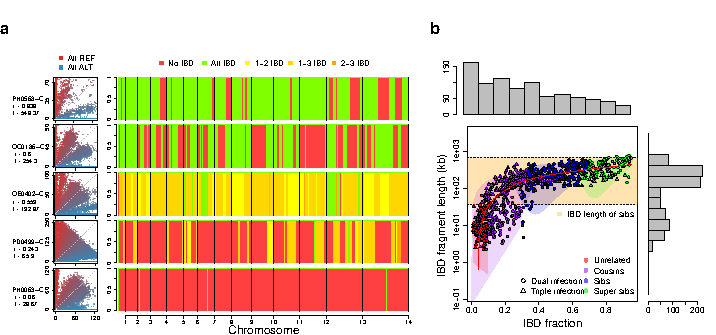
\includegraphics[width=\textwidth]{Fig3.pdf}
    \caption{Characterisation of mixed infections across 2,344 field samples of {\it Plasmodium falciparum}. (a) The fraction of samples, by population, inferred to carry one (clonal), two, three, or more than three strains.  Populations are ordered by rate of mixed infections within continent. We use shaded regions to indicate the distribution of 787 samples that, due to complex mixing or lack of data, had at least one low-quality deconvolved haplotype (note that filtering out those samples would underestimate the number of mixed strains). (b) The spectrum of IBD within mixed infections (including dual, triple and quad infections), broken down into unrelated (where the fraction of the genome inferred to be IBD, $r$, is $< 0.1$), low IBD ($0.1 \geq r < 0.3)$, sib-level ($0.3 \geq r<0.7$) and high ($r \geq 0.7$). Stars indicate the average.  Populations follow the same order as in panel a.  (c) The correlation between rates of mixed infection and level of identity by descent. Populations coloured by continent and showing $\pm 1$ s.e.m..  The dotted line shows the slope of the regression from a linear model.  Abbreviations: SN-Senegal, GM-The Gambia, NG-Nigeria, GN-Guinea, CD-The Democratic Republic of Congo, ML-Mali, GH-Ghana, MW-Malawi, MM-Myanmar, TH-Thailand, VN-Vietnam, KH-Cambodia, LA-Laos, BD-Bangladesh.} \label{fig:mixInfPlot}
  \end{center}
\end{figure}

Relatedness between samples and populations also varies substantially.  In dual infections, the average fraction of the genome inferred to be IBD ranges from 21\% in Guinea to 59\% in West Cambodia (Figure~\ref{fig:mixInfPlot}b). The mean relatedness inference is robust: it shows very strong correlation (0.95) before and after filtering out samples with poor haplotypes.  Asian populations show, on average, a higher level of relatedness within dual infections (48\%) compared to African populations (29\%).  Levels of IBD in samples with three or more strains are comparable to those seen in dual infections (average IBD being 50\% in Asia and 29\% in Africa) and significantly correlated (P = 0.0012) [correlated with WHAT?], except Senegal.  Overall, 53\% of all mixed infections involve strains with over 30\% of the genome being IBD (the 2.5th percentile of the IBD fraction distribution between true siblings, given the recombination rate in {\it P. falciparum}).

In general, we find that populations with higher rates of mixed infection tend to have lower levels of IBD in mixed infections (linear model P = 0.06 after accounting for a continental level difference and weighted by sample size).  However, the continental level effect is driven by Senegal, which has an unusual combination of low mixed infections, but also low IBD.  Excluding this population (see below for addition discussion), we find a consistent pattern across populations (Figure~\ref{fig:mixInfPlot}c), with a strong negative effect of mixed infection rate on level of IBD (P = $3\times10^{-4}$).

%The observed levels of IBD suggest that a substantial fraction of mixed infections involve sibling strains; those related through meiosis from distinct parental strains within a multiply-infected mosquito.  To further investigate this hypothesis, we examined the length distribution of IBD segments within mixed infections and compared these to observations from sibling strains generated through experimental lab crosses.  Figure~\ref{fig:strainIBD} shows examples of genomic IBD profiles in dual and triple infections.  In lab crosses cross-over events occur typically 200~kb to 1~Mb apart \citet{Miles2016}, hence IBD tracts are expected to be about half this length in dual sibling infections, and one third of this in triple infections (Figure~\ref{fig:strainIBD}).  By jointly considering IBD fraction and IBD length, we observe bimodal distributions of both variables, which can be used to identify mixed infections related to different degrees.  In this regard, we can identify those likely to be siblings from unrelated parents, siblings from related parents (i.e. with inbreeding) and strains separated by two to three meioses (Figure~\ref{fig:strainIBD}).  For example, we estimated that 23\% of dual infections carry sibs in Africa, whereas 25\% do so in Asia.%


\subsection{IBD patterns allow for classification of sibling mixed infections}


The high levels of IBD observed in many mixed infections were suggestive of a sibling relationship between constituent strains. To characterise the expected IBD patterns between siblings, we constructed a simulation of meiosis ({\tt pf-meiosis}), incorporating salient features of malaria biology that can impact the way IBD is produced in a mosquito and detected in a human host. Most prominently, a single infected mosquito can undergo multiple meioses in parallel --- one occurring for each oocyst that forms on the mosquito midgut.  In a mosquito infected with two distinct strains, each oocyst can be either selfed (the maternal and paternal strain are the same) or outbred (the maternal and paternal strains are different). We model a $k=n$ mixed infection as a sample of $n$ strains (without replacement, as drawing identical strains yields $k=n-1$) from the pool of strains created by all oocysts. Most studies suggest that the distribution of oocysts is roughly exponential with a mean of 1.5, implying that the most common number of oocysts in an infected mosquito is one. Interestingly, in such a case, a $k=2$ infection will have an expected IBD of $1/3$. Conditioning on at least one progeny from an outbred oocyst (such that a detectable recombination event has occurred), the expected IBD asymptotically approaches $1/2$ as the total number of oocysts grows.

Using this simulation framework, we sought to classify observed mixed infections based on their patterns of IBD. We used two summary statistics to perform the classification: mean IBD segment length and IBD fraction. We built distributions for these two statistics for each country in Pf3k, by simulating meiosis between pairs of clonal samples from that country.  In this way, we control for variation in genetic diversity (as latent IBD between clonal samples) in each country. Starting from a pair of clonal samples ($M=0$, where $M$ indicates the number of meioses that have occurred), we simulated three successive rounds of meiosis ($M=1, 2, 3$), representing the creation and serial transmission of a mixed infection (Figure~\ref{fig:classify}a). Each round of meiosis increases the amount of observed IBD, as segregation and recombination allow for portions of identity, generated during DNA replication, to end up in the progeny. For example, in Ghana, the mean IBD fraction for $M=0$ was 0.002, for $M=1$ was 0.41, for $M=2$ was 0.66, and for $M=3$ was 0.80 (Figure~\ref{fig:classify}b). West Cambodia, which has lower genetic diversity, had a mean IBD fraction of 0.08 for $M=0$ and consequently, the mean IBD fractions for higher values of $M$ were slightly increased, to 0.46, 0.68, 0.81 for $M=1, 2$ and $3$, respectively (Figure~\ref{fig:classify}b).

From these simulated distributions, we used Naive Bayes to classify all $k=2$ mixed infections in Pf3k (Figure~\ref{fig:classify}c).  Of the 404 samples with $k=2$, 288 (71\%) had IBD statistics that fell within the range observed across all $M$ in the simulation. Interestingly, more than half (221, 55\%) of all $k=2$ mixed infections were classified as siblings ($M > 0$, with > 99\% likelihood).  Moreover, we observe evidence for geographical differences in the rate at which sibling and unrelated mixed infections occur. Notably, in Asia, a greater fraction of all mixed infections contained siblings (65\% vs. 51\% in Africa), driven by a pronounced higher frequency of $M=2$ and $M=3$ mixed infections (Figure~\ref{fig:classify}d).


\begin{figure}[h]
  \begin{center}
  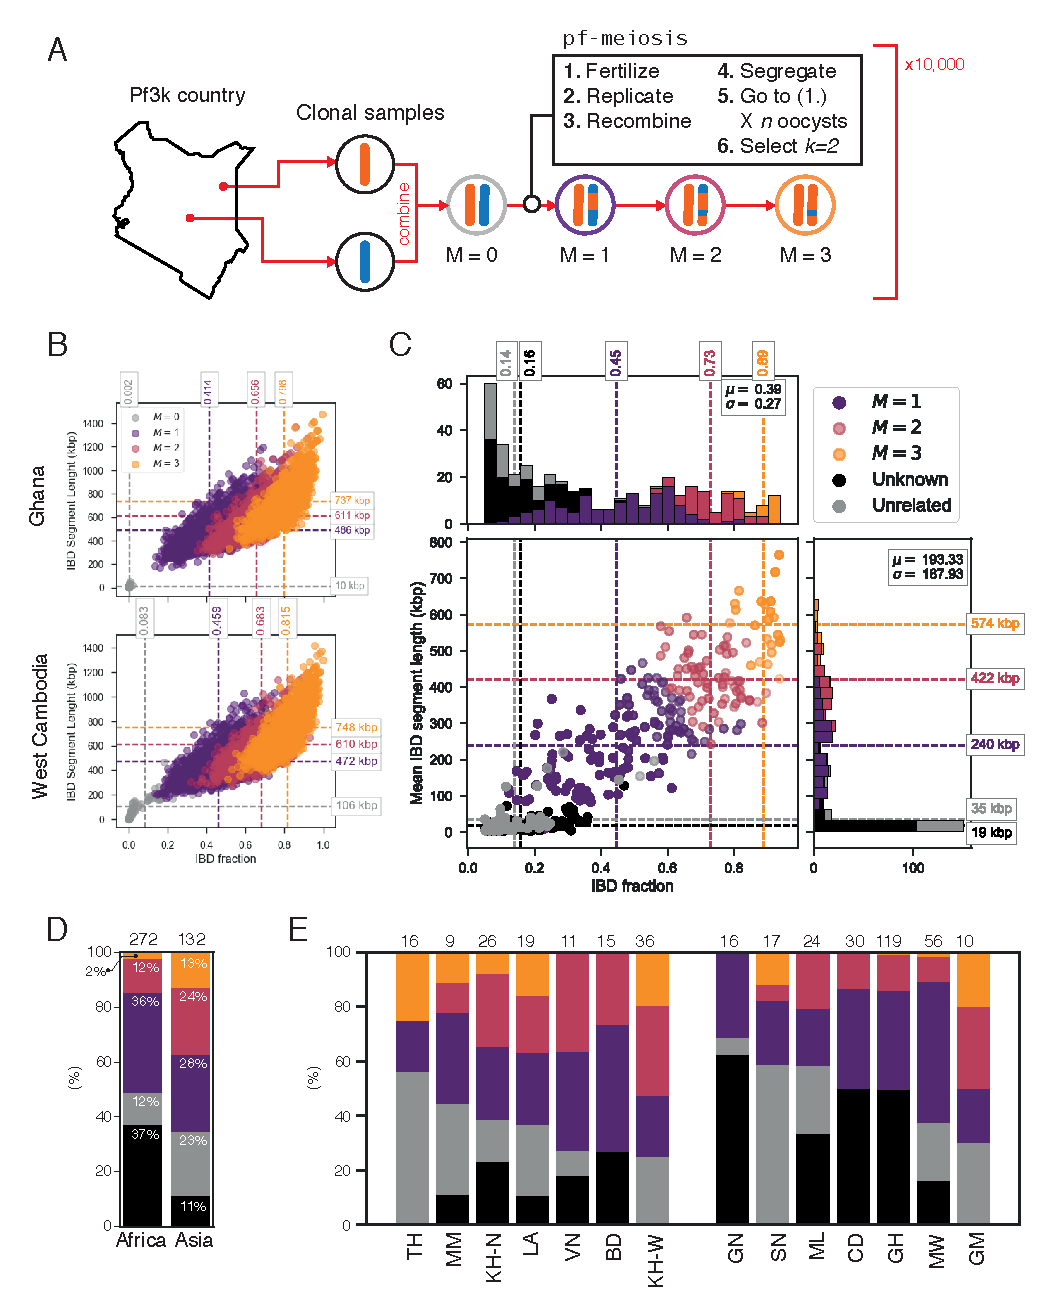
\includegraphics[width=\textwidth]{figures/Fig4-v3.pdf}
   \caption{Identifying sibling strains within mixed infections.  (a) Generating IBD fraction and segment length distributions for unrelated ($M=0$, grey), sibling ($M=1$, purple), inbred-sibling ($M=2$, pink) and doubly-inbred-sibling ($M=3$, orange) mixed infections. Two clonal samples from a given country are combined to produce a $K=2$ unrelated mixed infection which recapitulates local latent IBD. This unrelated infection is then passed through $n$ rounds of `pf-meioses` a malaria-specific meioses simulator, to generate $M=n$ classes. (b) Simulated IBD distributions for $M=0...3$ for Ghana and West Cambodia. A total of 10,000 examples are simulated for each class (c) Classification result of 404 $k=2$ mixed infections from 14 countries. Unknown indicates mixed infections with IBD statistics that were never observed by simulation. (d) Breakdown of class percentage by continent. Total number of samples is given above bars. (e) Breakdown of class percentage by country. Abbreviations: SN-Senegal, GM-The Gambia, NG-Nigeria, GN-Guinea, CD-The Democratic Republic of Congo, ML-Mali, GH-Ghana, MW-Malawi, MM-Myanmar, TH-Thailand, VN-Vietnam, KH-Cambodia, LA-Laos, BD-Bangladesh.} \label{fig:classify}
   \end{center}
   %\figsupp{IBD chunk lengths from crosses.}{\includegraphics[width=\textwidth]{Fig4Sup.pdf}}
\end{figure}

\subsection{Characteristics of mixed infections correlate with local parasite prevalence}


To assess how characteristics of mixed infection relate to local infection intensity, we obtained estimates of {\it P. falciparum} prevalence from the Malaria Atlas Project (MAP).  MAP provides smoothed estimates of prevalence, as well as summaries of the individual studies that are used to build the map. The smoothed estimates of prevalence  range from 0.01\% in Thailand to 55\% in Ghana, with African countries having over three orders of magnitude greater average infection intensity (mean of 30\% in Africa and 0.4\% in Asia). However, seasonal and geographic fluctuations in prevalence mean that, conditional on sampling an individual with malaria, local prevalence may be much higher than the longer-term (and more geographically widespread).  We therefore estimated a conditional prevalence, by excluding reports with zero positive results (see Table~\ref{tab:Pf3k}.
 We summarise mixed infection rates by the average effective number of strains (see above), which reflects both the number and proportion of strains present.  This metric both avoids the problem of having to determine a threshold for determining the presence of a very low proportion strain and is sensitive to the presence of triply (and more) infected samples.

After accounting for between-continent differences in prevalence, the effective number of strains is a significant predictor of local prevalence (linear model P = $1.62 \times 10^{-5}$), though the level of relatedness is not ($P>0.34$), either by itself or in combination with the rate of mixed infection (Figure~\ref{fig:model}~(d)).  The relationship between mixed infection rate and prevalence is driven entirely by the African populations ($P = 0.0004$).  Within the Asian populations, mixed infection rate is an extremely poor predictor of country-level prevalence ($P = 0.23$).

Two features stand out from this analysis.  First, despite having orders of magnitude difference in {\it P. falciparum} prevalence at the country level, rates of mixed infection in Asian populations are typically within a factor of two of those in African populations.  This observation is particularly surprising given the association between mixed infection rate and prevalence within African populations and could point to either substantial heterogeneity in local transmission rates within Asian populations or an unexpected consequence of malaria epidemiology.  Second, given the (negative) association between mixed infection rate and levels of IBD, it seems unexpected that levels of IBD do not correlate with prevalence at the country level but this could be partially explained by the marked differences in the distribution of background IBD among countries (i.e. relatedness between strains found in different isolates).



%To better understand the expected relationships between pathogen prevalence and statistics of infection, we developed a simple extension of the classic Ross-MacDonald model \citep{Smith2012} of malaria transmission to include mixed infection within both hosts and vectors (Figure~\ref{fig:model}). In this deterministic model, we assume a fixed number of hosts and vectors, that infection status does not affect probability of transmission or sampling and that the bottlenecks at transmission to host or vector can be approximated as a single parameter that determines the probability that a multiply-infected host (or vector) transmits more than one strain (if they are themselves multiply-infected.  See Supplementary Material for model details.  At equilibrium, this model recovers the standard relationship between vector density and/or biting rate and local prevalence: $\pi = (\lambda_H - \gamma \xi)/(\lambda_H + \lambda \xi)$, where $\lambda_H$ is the expected number of bites per host per day that could lead to infection, $\gamma$ is the rate of host clearance, and $\xi$ is the rate of vector replacement (or clearance) .  However, in addition, we  can predict how mixed infection rates covary with prevalence and, in addition, approximate the relative contribution of sib-infections by comparing the contribution to novel mixed infections, at equilibrium, from previously uninfected hosts (hence infected by a single multiply-infected mosquito, assumed to transmit sibling strains, occurring at rate $H_0 V_M \lambda_H \phi$) and from previously singly-infected strains (hence carrying at least two distinct strains, occurring at rate $H_1 (V_1 + V_M) \lambda_H$).  This model has several limitations, for example not being able to model background levels of relatedness, but nevertheless serves as a useful indicator of how more complex and realistic models might behave.  We note that the model does not consider the effective number of strains directly, however, we expect a monotonic relationship with mixed infection rate.%

%Analysis of the model reveals two features.  First, by altering the vector population, the rate of mixed infection tracks prevalence in a largely linear manner, though at high prevalence, there is a somewhat greater than linear relationship, see Figure~\ref{fig:model}b.  Second, the relative contribution of sibling strains (compared to unrelated strains) in mixed infections is relatively constant across varying prevalence, with the exception of a  high contribution at very low prevalence (Figure~\ref{fig:model}b).  These observations are consistent with the genomic data presented here (Figure~\ref{fig:model}), where we see significant correlation between prevalence and mixed infection, but no significant correlation with relatedness in mixed infections (despite the negative correlation between mixed infection rate and IBD fraction).  Figure~\ref{fig:model}b shows a choice of parameter values that broadly match the empirical data.  These results suggest that rates of mixed infection are likely to be highly informative about the local intensity of {\it P. falciparum} transmission.  In contrast, the relative contribution of sibling infection to mixed infections reflects fundamental parameters relating to transmission events.%


\begin{figure}[h]
  \centering{}
  \includegraphics[width=.6\textwidth]{Fig5.pdf}
  \caption{The relationship between {\it P. falciparum} prevalence and characteristics of mixed infection. For each sampling country and year, the relationship between the average effective number of strains, given by $(\sum f_i^2)^{-1}$, where $f_i$ is the proportion of the $i$th strain and the estimated prevalence.  Point shape indicates country and colour indicates the average level of IBD observed within mixed infections. Point size is proportional to Pf3k sample size.}
  \label{fig:model}
\end{figure}


\section{Discussion}

Genome sequencing of malaria parasites obtained from human hosts has revealed many striking features of malaria evolution and population structure. Some of these discoveries comprise the repeated origin of artemisinin resistance mutations in South East Asia \citep{miotto2015genetic}, high levels of population differentiation \citep{Miotto2013}, and the presence of many loci that show evidence for adaptive evolution or long-term balancing selection [REF].  However, the extent to which such data can give high resolution information about malaria epidemiology, in both space and time, and thus inform control strategies, is largely unknown.  Here, we have focused on the problem of learning about mixed infections from genome-sequencing data.  Mixed infections have been studied previously \citep{Galinsky2015}, \citep{Jack2016}, \citep{auburn2012characterization}, \citep{assefa2014estmoi}, but the tools developed here enable estimates, not only of the presence of multiple strains, but their proportions, relatedness, and haplotypes.  We have shown that, in the populations studied here, between 16\% and 63\% of isolates have multiple infections, and up to 51\% have more than two.  Perhaps most unexpected, we have also shown that over half of all mixed infections include strains related at the level of siblings, with chromosomal patterns of IBD that indicate progeny from a single infected mosquito.  Even in regions of extremely low average prevalence, such as in parts of South East Asia (for example Vietnam has a mean prevalence of less than 1 in 1,000 \citep{who2017, who2017profile}), where individuals infected with malaria are found, they frequently carry mixed infection (we estimate 31\%) and, again, often with sibling strains (75\% for Vietnam).

%To better understand how observations of characteristics of mixed infection relate to epidemiological processes, we introduced a simple deterministic model for mixed infection.  For a given set of transmission parameters (those relating to the relative chances of transmitting single and multiple strains at host-vector interactions), as vector density increases, so does prevalence and, in a roughly linear manner, the expected mixed infection rate.  Consequently, the order of magnitude differences in prevalence seen between Asian and African populations would be expected to translate into orders of magnitude differences in mixed infection rate. That this is not observed points either to differences in the biology of transmission (for example resulting from differences in vector biology) or to heterogeneity of transmission within Asian populations, with hotspots of transmission (in both space and possibly time). Transmission hotspots are highly seasonal \citep{Ahmed2013}.%

In both Africa \citep{Bejon2010} and Asia \citep{Heng2017}, researchers have identified stable hotspots last for several years and unstable hotspots that disappears after one year or two. Nevertheless, within African populations mixed infection rate is a significant predictor of country-level prevalence, suggesting that the metric is a potentially useful source of information for measuring local transmission intensity.  We note that Senegal, where there has been a dramatic reduction in malaria prevalence \citep{Daniels2015}, is an outlier in terms of this metric within Africa (Figure~\ref{fig:mixInfPlot}).

%While many individuals with malaria carry mixed infections, in the majority of cases the parasite strains are related, often at the level of siblings or even greater.  That sibling strains are frequently observed (we estimate XX \% of all mixed infections) indicates that the transmission bottleneck from vector to host is relatively weak.  One route by which \'supersib\' infections could occur (i.e. sibs from parents that are themselves related) is through onward transmission of sibling strains in a host to a vector, with subsequent meiosis and transmission to a new host. Thus a single mosquito that acquired two distinct malaria strains through biting multiple infected hosts could potentially generate a chain of mixed infections, with increasing levels of IBD.  Such events are likely to play an important role particularly in low transmission settings, which is consistent with our observations of higher levels of IBD in Asian populations.  More generally, we can estimate relatedness both within infections and between infections as a route to identify groups of individuals that likely represent transmission chains.%


The approach presented here, combined with population-scale sequencing of pathogen genomes from those infected with malaria parasites, offers new tools for control programmes.  We have shown that simple metrics of mixed infection rate are predictive of current local prevalence and that relatedness patterns provide additional information about local dynamics.  However, there are many challenges to providing robust and meaningful predictions.  Perhaps most importantly, sampling strategies for obtaining pathogen genomes are likely to bias information in space and time.  The extent to which this will be problematic for quantitative inference is unknown and requires further investigation.  Other complications, such as whether the vector or host exerts a selective force on mixed infections that is distinct from single infections, or how prior (or current) infection influences the chances of subsequent infection, will also be important to determine to achieve better understanding of the mixed infection process.



\section{Acknowledgements}
The project is funded by  Wellcome (100956/Z/13/Z to GM, \ldots).


\section{Data availability}
Metadata on samples is available from \url{ftp://ngs.sanger.ac.uk/production/pf3k/release_5/pf3k_release_5_metadata_20170804.txt.gz}.  Sequence data (aligned to Plasmodium falciparum strain 3D7 v3.1 reference genome sequences, for details see \url{      ftp://ftp.sanger.ac.uk/pub/project/pathogens/gff3/2015-08/Pfalciparum.genome.fasta.gz}) is available from  \url{ftp://ngs.sanger.ac.uk/production/pf3k/release_5/5.1/}.  {\it P. falciparum} prevelance estimates were taken from \url{https://map.ox.ac.uk/country-profiles/#!/}.  Inferred haploytpes from each sample are available from XXX.


\section{Disclosure Declaration}
None declared.


\bibliography{mixedIBD.bib}


\end{document}
